\documentclass[a4paper,12pt]{article}

\usepackage{mathtext}
\usepackage[T2A]{fontenc}
\usepackage[utf8]{inputenc}
\usepackage[russian]{babel}
\usepackage{multirow}
\usepackage{slashbox}
\usepackage{makecell}
\usepackage{graphicx}
\usepackage{physics}
\usepackage{amstext}
\usepackage{caption}
\usepackage{subcaption}


\title{Лабораторная работа 3}
\author{Калашников Михаил, Б03-205}
\date{}


\begin{document}

\maketitle{Библиотеки, бинарники и оптимизация}

\begin{enumerate}

\setcounter{enumi}{0}

\item Соберем статическую библиотеку из файла sum\_x64.s, скомпилируем ее вместе с файлом base.c и откроем бинарник с помощью objdump. Найдем там функцию sum. При использовании динамической библиотеки в бинарнике присутствует только вызов самой функции sum.

\begin{figure}[h!]
  \centering
  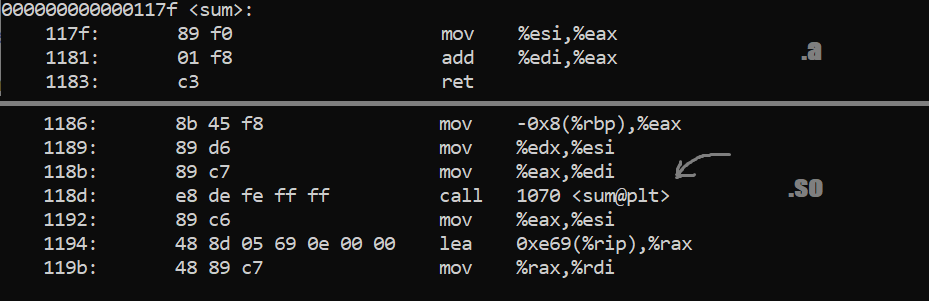
\includegraphics[width=0.8\linewidth]{images/asm3_1.png}
  \caption{К пункту 1}
\end{figure}

\item Напишем helloworld, скомпилируем и заглянем в бинарник. Там без труда можно найти строку hello world и отредачить нужные байты.

\begin{figure}[h!]
  \centering
  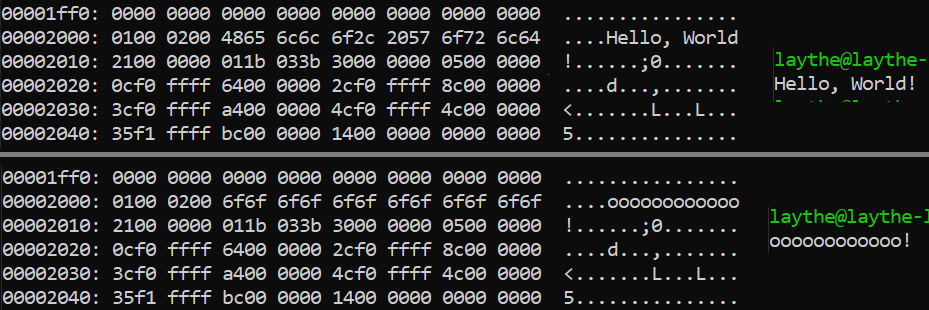
\includegraphics[width=0.8\linewidth]{images/asm3_2.png}
  \caption{К пункту 2}
\end{figure}

\item Теперь приступим к вскрытию бинарников. 

\begin{enumerate}

\item Пароль к первому можно без труда найти в через vim:
\[Ground\ control\ to\ major\ Tom,\ your\ circuit's\ dead,\]
\[there's\ something\ wrong.\]
Это строчка из песни Дэвида Боуи - Space Oddity.

\item Пароль от второго записан в бинарнике в обратном порядке. Перевернув его, получим пароль:
\[For\ so\ many\ years\ have\ gone,\ though\ I'm\ older\ but\ a\ year.\]
А это строчка из песни Queen - '39.

\item Уффф, третий файл. В нем имеется отрывок книги Харриса Роберта "Fatherland". Сравнив отрывок с оригиналом, можно заметить, что в отрывке имеются лишние слова. Написав скрипт, которые сравнит два куска текста и найдет различия, можно определить лишние слова: mankind, could, projections, We, past, salvage, this, into, to, send, use, the. Из этих слов явно можно составить предложение. Погуглив различные комбинации, можно найти что этот пароль является строчкой из песни Ayreon - $E=mc^2$:
\[We\ could\ use\ this\ to\ salvage\ mankind\]
\[ send\ projections\ into\ the\ past.\]

\item Пароль от четвертого пункта зашифрован шифром Цезаря со сдвигом на одну букву: 
\[Burn\ the\ land\ and\ boil\ the\ sea\ -\ you\ can't\ take\ the\ sky\ from\ me.\]
Строчка из песни Sonny Rhodes - Ballad of Serenity.

\item Пятый пункт зашифрован аналогично, только теперь сдвиг на две буквы. Пароль:
\[It's\ so\ enormously\ frightening\ when\ our\ tail\ reaches\ superheat.\]
Строчка из песни The Gathering - Liberty Bell.

\item Шестой странный. Тот же отрывок из книги что и в третьем пункте, только в конце предложение в шифре Цезаря со сдвигом в три буквы, которое и является паролем.
\[There\ is\ research\ to\ be\ done\ on\ the\ people\ who\ are\ still\ alive.\]
Строчка из очень красивой песни из титров первого Портала GlaDOS - Still Alive.

\item А вот седьмой интересный. В нем не простой шифр Цезаря, сдвиг каждого символа зависит от его индекса в строке и равен $(i\ \%\ 5) + 1$. Догадаться до этого было очень непросто. :( Собственно, пароль:
\[Disturbing\ thoughts,\ questions\ pending,\]
\[limitations\ of\ human\ understanding.\]
Является строчкой из песни метлы Through the Never.

\item Восьмой на удивление очень простой. Пароль просто лежит в бинарнике (???):
\[We're\ heading\ for\ Venus,\ and\ still\ we\ stand\ tall.\]
А это уже строчка из песни Europe - The Final Countdown.

\end{enumerate}

\end{enumerate}

\end{document}